% !TEX root = ../notes.tex














Ok so my keyboard is now working.

\subsection{Completions of Dedekind Domains}
Recall from last time we had the following statement.
\begin{proposition}
	Fix $A$ a Dedekind ring with $K$ its fraction field. Fix $\mf p$ a nonzero prime of $A,$ and let $\nu_\mf p:K\to\ZZ\cup\{\infty\}$ be the discrete valuation of $\mf p.$ Further fix $c>1$ and define
	\[|x|_\mf p:=c^{-\nu_\mf p(x)},\]
	where $x\in K.$ If we complete $(A,|\cdot|_\mf p)$ and $(K,|\cdot|_\mf p)$ to $(\hat A,|\cdot|^\wedge_\mf p)$ and $(K,|\cdot|_\mf p^\wedge)$ respectively, then we have the following.
	\begin{enumerate}[label=(\alph*)]
		\item There is a canonical isomorphism
		\[\hat A\cong\limit A/\mf p^\bullet.\]
		\item $\hat A$ is a discrete valuation ring with valuation $-\log_c|\cdot|_\mf p^\wedge$ and fraction field $\hat K.$
	\end{enumerate}
\end{proposition}
\begin{proof}
	We are showing part (b) now. We will now write $|\cdot|$ for all of our valuations because they extend properly. We have the following claims.
	\begin{lemma}
		For any non-archimedean valued ring $(R,|\cdot|),$ we have that $\{|\alpha|:\alpha\in\hat R\}=\{|\alpha|:\alpha\in R\}.$
	\end{lemma}
	\begin{proof}
		Note that $R$ embeds into $\hat R,$ so of course we get $\supseteq.$ For $\subseteq,$ we suppose that we have a Cauchy sequence $(a_0,a_1,\ldots)$ approaching some $\alpha.$ Then there exists $N$ for which
		\[|a_i-a_j|<\alpha\]
		for each $i,j\ge N$ because $\alpha\ne0.$ But then this implies that $|\alpha|=|a_i|$ for each $i\ge N,$ so it follows that $|\alpha|\in\{|a|:a\in R\}.$
	\end{proof}
	\begin{lemma}
		Fix everything as above The function $\nu:\alpha\mapsto-\log_c|\alpha|$ is a discrete valuation on $\hat K.$
	\end{lemma}
	\begin{proof}
		The fact that $\nu(x+y)=\nu(x)+\nu(y)$ follows from the multiplicativity of absolute values. We also have tht the range of $|\cdot|$ on $\hat K$ is its range on $K$ from the previous claim. We leave the check of the strong triangle inequality as an exercise.
	\end{proof}
	\begin{lemma} \label{lem:something}
		Fix everything as above. Then the valuation ring of $\nu$ is $\hat A.$
	\end{lemma}
	\begin{proof}
		We see that $\hat A$ is in the valuation ring because the image of $\hat A$ under $|\cdot|$ is the image of $A,$ so indeed, $\hat A$ has nonnegative valuation.

		In the other direction, suppose that $\alpha\in\hat K$ has $\nu(\alpha)\ge0$ so that $|\alpha|\le1.$ Then we can make $\alpha$ into a Cauchy sequence $(a_0,a_1,\ldots)$ in $K,$ and now we take $N$ as we did before so that $i\ge N$ implies $|a_i|=|\alpha|.$ The point is that
		\[|a_i|=|\alpha|\le1\]
		for each $i\ge N,$ which means that the $a_i\in A_\mf p,$ so we may represent $\alpha$ by the Cauchy sequence
		\[(a_N,a_{N+1},a_{N+2},\ldots)\in\limit A_\mf p/(\mf pA\mf p)^\bullet=\limit A/\mf p^\bullet=\hat A.\]
		The middle equality deserves some explanation: we have that $A_\mf p/(\mf pA_\mf p)^\bullet=(A\setminus\mf p)^{-1}(A/\mf p^\bullet),$ but the $A\setminus\mf p$ will add no new units to $A/\mf p^\bullet,$ so it is simply $A/\mf p^\bullet.$
	\end{proof}
	\begin{remark}
		Alternatively, we could have noted that $A_\mf p$ injects into $\hat A$ so that $\alpha$ living in the completion of $A_\mf p$ makes $\alpha$ live in $\hat A.$
	\end{remark}
	We finish by noting that it follows $\hat A$ is a discrete valuation ring because it is a valuation ring of the discrete valuation $\nu.$ This finishes the proof.
\end{proof}
We note that from the above we get that $\hat K$ is the fraction field of $\hat A,$ and we are granted the unique maximal ideal
\[\hat m:=\{\alpha\in\hat A:\nu(\alpha)\ge1\}.\]
In fact, we can note that some $\pi\in\mf p\setminus\mf p^2$ will give $\hat m=\pi\hat A,$ where
\[A/\mf p^\bullet\to\hat A/(\pi^\bullet)=\hat A/\hat m^\bullet\]
is an isomorphism. This more or less follows from our argument earlier for \autoref{lem:something}. \todo{wut}
\begin{example}
	Fix $k$ a field and $A=k[x]$ with $K=k(x)$ and $\mf p=(x).$ Then $\hat A=k[[x]]$ and $\hat K=k((x)).$
\end{example}
We also remark that, in general,
\[\hat K=\bigcup_{n\ge 0}\pi^{-n}\hat A\]
for any Dedekind domain $A.$

\subsection{Topological Remarks}
We note that if $k$ is infinite, then $k[[x]]$ is not compact (sadly):
\[\{c+(x):c\in k\}\]
is a disjoint open cover of $k[[x]].$ But $\ZZ_p$ is compact, as will be shown in the homework.

As an image, we can see $\ZZ_3$ as follows.
\begin{center}
	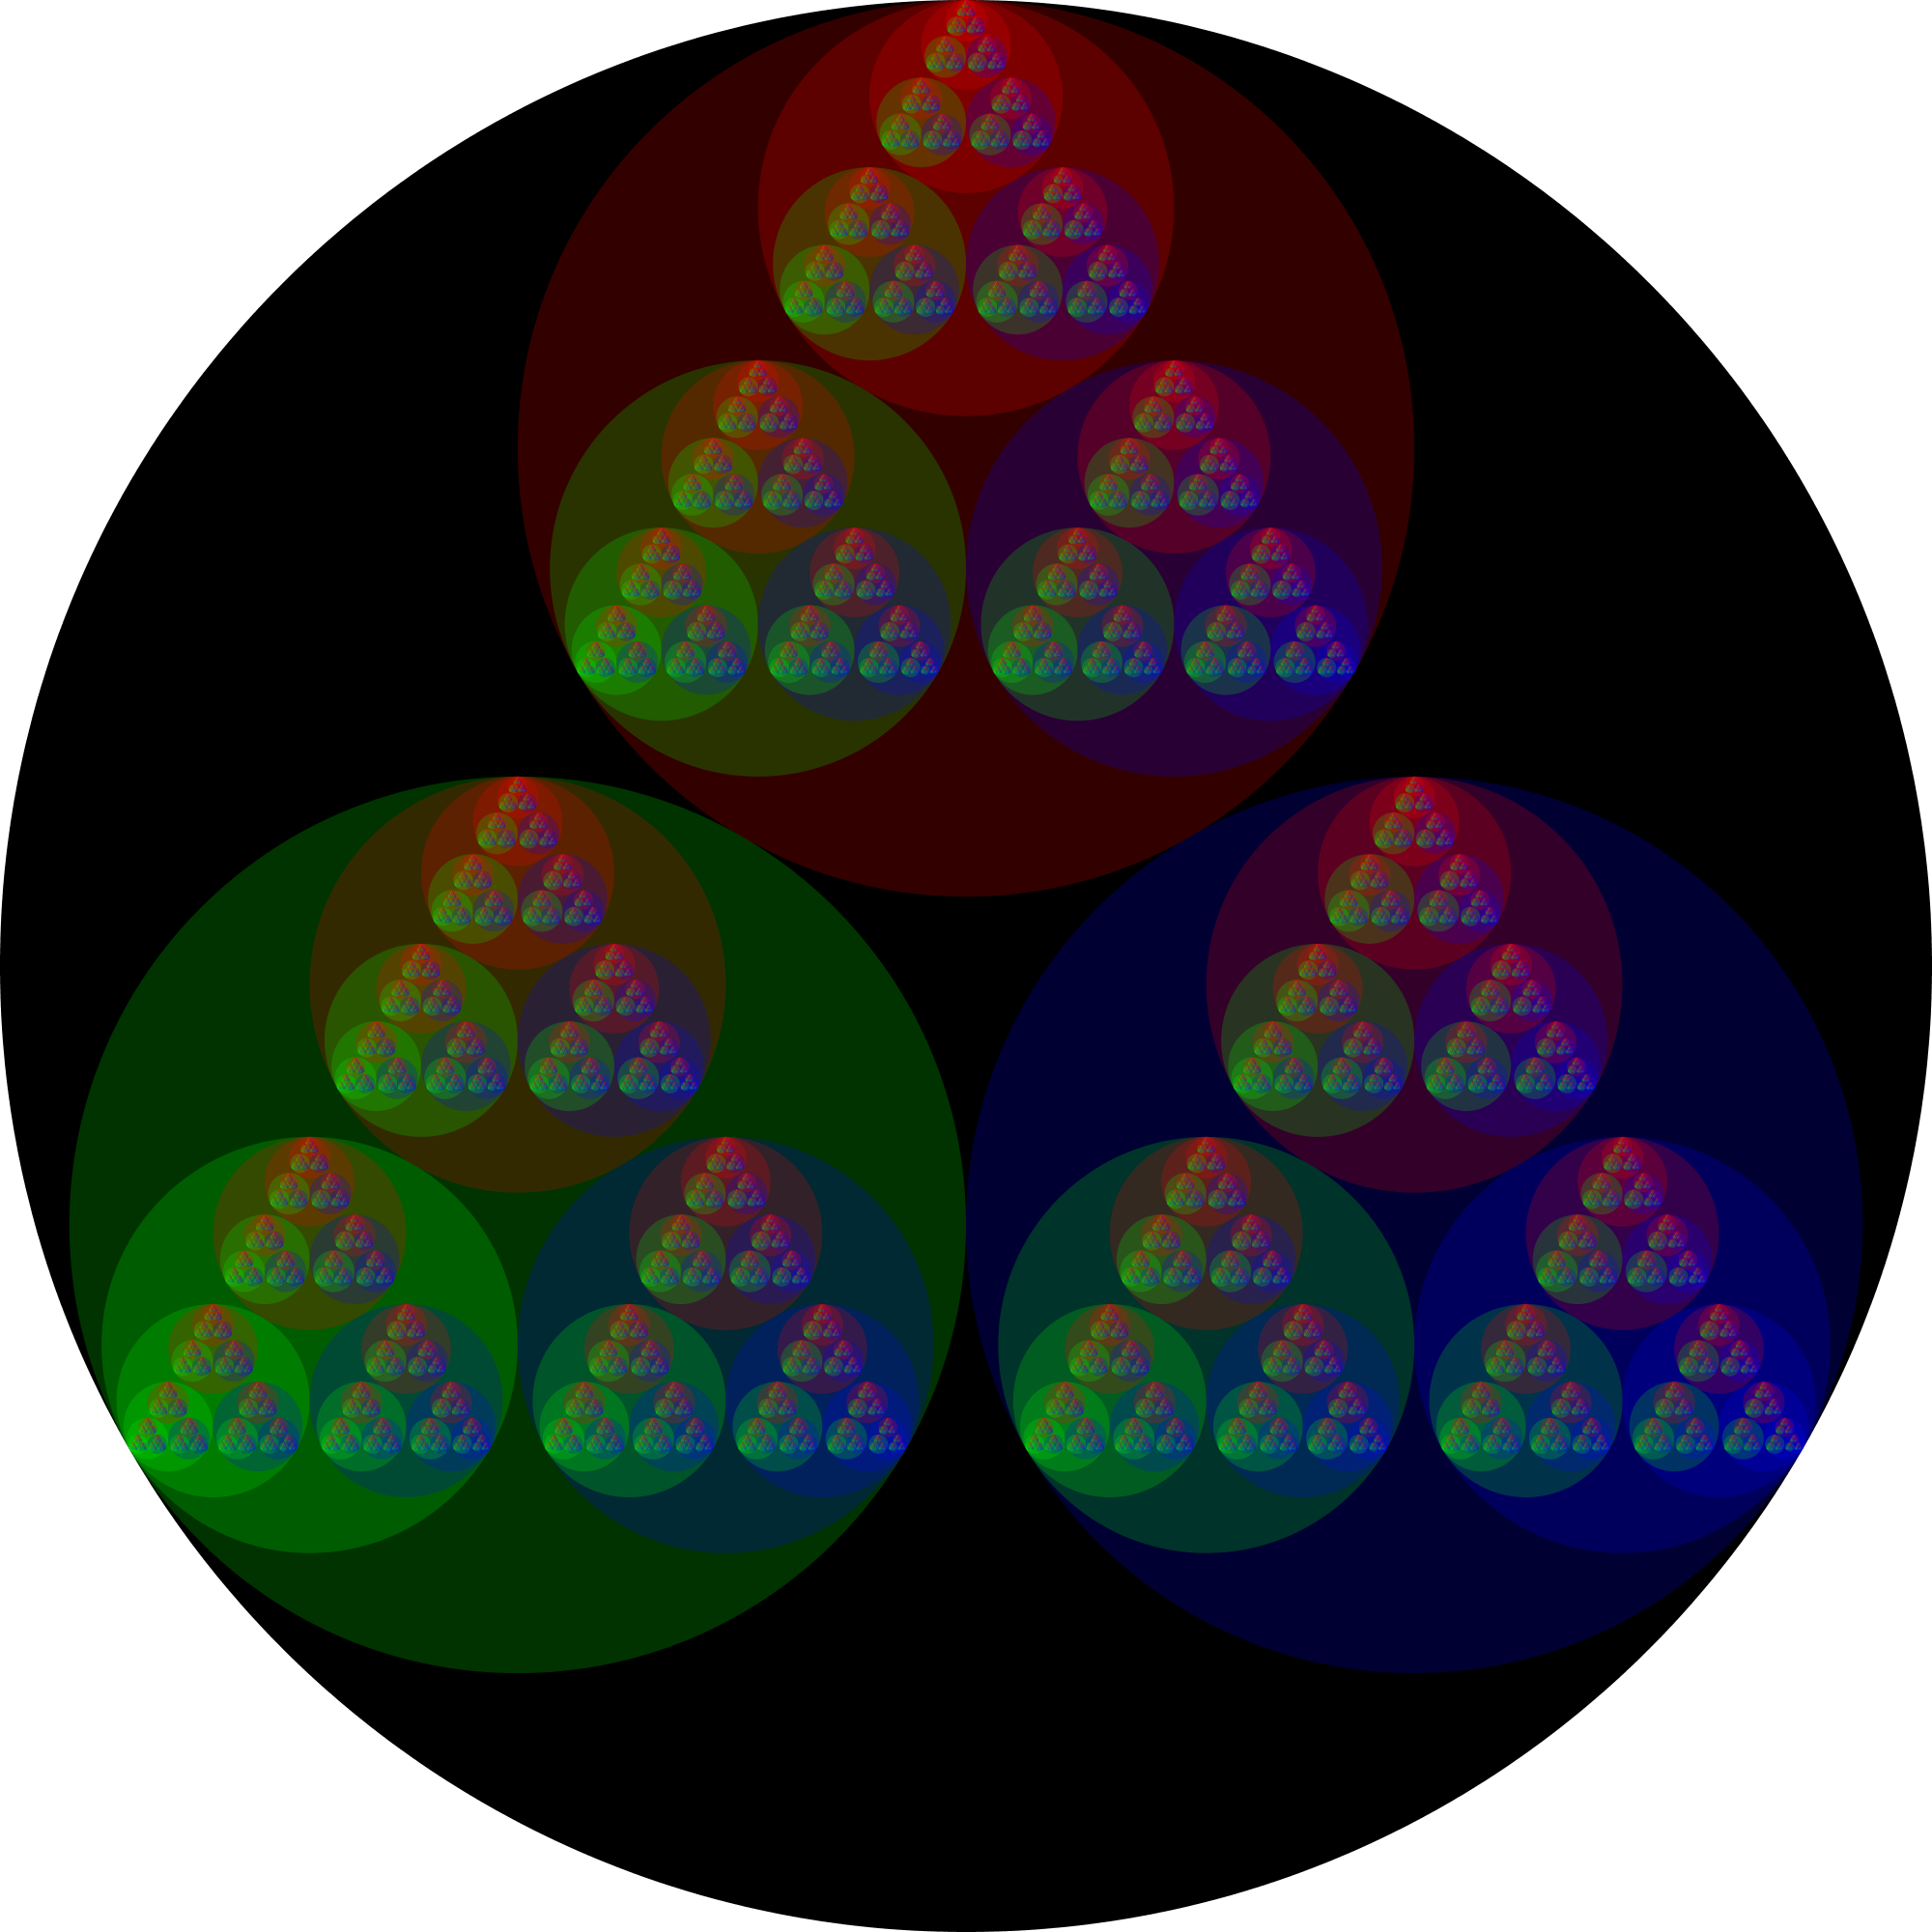
\includegraphics[scale=0.1]{./3-adics-dark.png}
\end{center}
Each circle here corresponds to successively smaller residue classes. More generally, $\hat A$ where $A$ is non-archimedean will make $\hat A$ totally disconnected.

As an aside, we note that we can let $k$ be an arbitrary field, not necessarily algebraically closed. Then with $A=k[x],$ we have that the set of nonzero of nonzero prime ideals of $A$ is in bijection with the monic irreducible ideals of $k[x]$ by $\pi\mapsto(\pi).$ Then if we let
\[M_k=\{\infty\}\cup\{(\pi):\pi\in k[x]\text{ irred.}\},\]
we get a $|\cdot|_\nu$ for each place $\nu\in M_K,$ induced by $|x|_\mf p:=c^{-(\deg f)\nu_\mf p(x)}$ for some $c>1.$ Then we have the product formula given by
\[\prod_{\mf p\in M_K}|x|_\mf p=1\]
for each $x\in k(x)^\times.$ Again, this is essentially by unique prime factorization.

\subsection{Valuations}
Yes, we have been talking about valuations already. Let's talk some more.
\begin{definition}[Trivial]
	An absolute value $|\cdot|$ is \textit{trivial} if and only if $|x|=1$ for each $x\in R\setminus\{0\}$ and nontrivial otherwise.
\end{definition}
\begin{remark}
	The trivial valuation is non-archimedean: it corresponds with the valuation sending everything nonzero to $0.$
\end{remark}
The trivial absolute value is a perfectly fine valuation, but we don't want to have to care about it.

We have the following.
\begin{proposition}
	Fix $(R,|\cdot|)$ a valued ring. Then the following are equivalent.
	\begin{enumerate}[label=(\alph*)]
		\item $R$ is non-archimedean.
		\item $|n|\le1$ for each $N\in\ZZ.$
		\item $\{|n|:n\in\ZZ\}$ is a bounded set.
	\end{enumerate}
\end{proposition}
\begin{proof}
	We show our implications one at a time.
	\begin{itemize}
		\item We get that (a) implies (b) by an induction. If $R=\{0\},$ then this is free; otherwise, $|1|=1$ and then, for $n\in\NN,$
		\[|\pm n|=|n|=|\underbrace{1+\cdots+1}_n|\le\max\{\underbrace{|1|,\ldots,|1|}_n\}=1\]
		by the strong triangle inequality.
		\item We see that (b) implies (c) by definition of bounded.
		\item We see that (c) implies (a): suppose that $|n|\le L$ for each $n\in\ZZ.$ Then, taking any $x,y\in R,$ we find that
		\[|x+y|^n=\left|\sum_{k=0}^n\binom nkx^ky^{n-k}\right|\le\sum_{k=0}^n\left|\binom nk\right|\cdot\max\{|x|,|y|\}^n\le(n+1)L\max\{|x|,|y|\}^n.\]
		In particular, we see that
		\[|x+y|\le\sqrt[n]{(n+1)L}\cdot\max\{|x|,|y|\},\]
		so it follows that
		\[|x+y|\le\max\{|x|,|y|\}\cdot\limsup_{n\to\infty}\sqrt[n]{(n+1)L}=\max\{|x|,|y|\},\]
		which is what we wanted.
		\qedhere
	\end{itemize}
\end{proof}